\documentclass[11pt,preprint]{elsarticle}

\usepackage{lmodern}
%%%% My spacing
\usepackage{setspace}
\setstretch{1.2}
\DeclareMathSizes{12}{14}{10}{10}

% Wrap around which gives all figures included the [H] command, or places it "here". This can be tedious to code in Rmarkdown.
\usepackage{float}
\let\origfigure\figure
\let\endorigfigure\endfigure
\renewenvironment{figure}[1][2] {
    \expandafter\origfigure\expandafter[H]
} {
    \endorigfigure
}

\let\origtable\table
\let\endorigtable\endtable
\renewenvironment{table}[1][2] {
    \expandafter\origtable\expandafter[H]
} {
    \endorigtable
}


\usepackage{ifxetex,ifluatex}
\usepackage{fixltx2e} % provides \textsubscript
\ifnum 0\ifxetex 1\fi\ifluatex 1\fi=0 % if pdftex
  \usepackage[T1]{fontenc}
  \usepackage[utf8]{inputenc}
\else % if luatex or xelatex
  \ifxetex
    \usepackage{mathspec}
    \usepackage{xltxtra,xunicode}
  \else
    \usepackage{fontspec}
  \fi
  \defaultfontfeatures{Mapping=tex-text,Scale=MatchLowercase}
  \newcommand{\euro}{€}
\fi

\usepackage{amssymb, amsmath, amsthm, amsfonts}

\def\bibsection{\section*{References}} %%% Make "References" appear before bibliography


\usepackage[numbers]{natbib}

\usepackage{longtable}
\usepackage[margin=2.3cm,bottom=2cm,top=2.5cm, includefoot]{geometry}
\usepackage{fancyhdr}
\usepackage[bottom, hang, flushmargin]{footmisc}
\usepackage{graphicx}
\numberwithin{equation}{section}
\numberwithin{figure}{section}
\numberwithin{table}{section}
\setlength{\parindent}{0cm}
\setlength{\parskip}{1.3ex plus 0.5ex minus 0.3ex}
\usepackage{textcomp}
\renewcommand{\headrulewidth}{0.2pt}
\renewcommand{\footrulewidth}{0.3pt}

\usepackage{array}
\newcolumntype{x}[1]{>{\centering\arraybackslash\hspace{0pt}}p{#1}}

%%%%  Remove the "preprint submitted to" part. Don't worry about this either, it just looks better without it:
\makeatletter
\def\ps@pprintTitle{%
  \let\@oddhead\@empty
  \let\@evenhead\@empty
  \let\@oddfoot\@empty
  \let\@evenfoot\@oddfoot
}
\makeatother

 \def\tightlist{} % This allows for subbullets!

\usepackage{hyperref}
\hypersetup{breaklinks=true,
            bookmarks=true,
            colorlinks=true,
            citecolor=blue,
            urlcolor=blue,
            linkcolor=blue,
            pdfborder={0 0 0}}


% The following packages allow huxtable to work:
\usepackage{siunitx}
\usepackage{multirow}
\usepackage{hhline}
\usepackage{calc}
\usepackage{tabularx}
\usepackage{booktabs}
\usepackage{caption}


\newenvironment{columns}[1][]{}{}

\newenvironment{column}[1]{\begin{minipage}{#1}\ignorespaces}{%
\end{minipage}
\ifhmode\unskip\fi
\aftergroup\useignorespacesandallpars}

\def\useignorespacesandallpars#1\ignorespaces\fi{%
#1\fi\ignorespacesandallpars}

\makeatletter
\def\ignorespacesandallpars{%
  \@ifnextchar\par
    {\expandafter\ignorespacesandallpars\@gobble}%
    {}%
}
\makeatother


% definitions for citeproc citations
\NewDocumentCommand\citeproctext{}{}
\NewDocumentCommand\citeproc{mm}{%
\begingroup\def\citeproctext{#2}\cite{#1}\endgroup}
\makeatletter
% allow citations to break across lines
\let\@cite@ofmt\@firstofone
% avoid brackets around text for \cite:
\def\@biblabel#1{}
\def\@cite#1#2{{#1\if@tempswa , #2\fi}}
\makeatother
\newlength{\cslhangindent}
\setlength{\cslhangindent}{1.5em}
\newlength{\csllabelwidth}
\setlength{\csllabelwidth}{3em}
\newenvironment{CSLReferences}[2] % #1 hanging-indent, #2 entry-spacing
{\begin{list}{}{%
	\setlength{\itemindent}{0pt}
	\setlength{\leftmargin}{0pt}
	\setlength{\parsep}{0pt}
	% turn on hanging indent if param 1 is 1
	\ifodd #1
	\setlength{\leftmargin}{\cslhangindent}
	\setlength{\itemindent}{-1\cslhangindent}
	\fi
	% set entry spacing
	\setlength{\itemsep}{#2\baselineskip}}}
{\end{list}}

\usepackage{calc}
\newcommand{\CSLBlock}[1]{\hfill\break\parbox[t]{\linewidth}{\strut\ignorespaces#1\strut}}
\newcommand{\CSLLeftMargin}[1]{\parbox[t]{\csllabelwidth}{\strut#1\strut}}
\newcommand{\CSLRightInline}[1]{\parbox[t]{\linewidth - \csllabelwidth}{\strut#1\strut}}
\newcommand{\CSLIndent}[1]{\hspace{\cslhangindent}#1}


\urlstyle{same}  % don't use monospace font for urls
\setlength{\parindent}{0pt}
\setlength{\parskip}{6pt plus 2pt minus 1pt}
\setlength{\emergencystretch}{3em}  % prevent overfull lines
\setcounter{secnumdepth}{5}

%%% Use protect on footnotes to avoid problems with footnotes in titles
\let\rmarkdownfootnote\footnote%
\def\footnote{\protect\rmarkdownfootnote}
\IfFileExists{upquote.sty}{\usepackage{upquote}}{}

%%% Include extra packages specified by user
\usepackage{lscape}\usepackage{booktabs}
\usepackage{longtable}
\usepackage{array}
\usepackage{multirow}
\usepackage{wrapfig}
\usepackage{float}
\usepackage{colortbl}
\usepackage{pdflscape}
\usepackage{tabu}
\usepackage{threeparttable}
\usepackage{threeparttablex}
\usepackage[normalem]{ulem}
\usepackage{makecell}
\usepackage{xcolor}

%%% Hard setting column skips for reports - this ensures greater consistency and control over the length settings in the document.
%% page layout
%% paragraphs
\setlength{\baselineskip}{12pt plus 0pt minus 0pt}
\setlength{\parskip}{12pt plus 0pt minus 0pt}
\setlength{\parindent}{0pt plus 0pt minus 0pt}
%% floats
\setlength{\floatsep}{12pt plus 0 pt minus 0pt}
\setlength{\textfloatsep}{20pt plus 0pt minus 0pt}
\setlength{\intextsep}{14pt plus 0pt minus 0pt}
\setlength{\dbltextfloatsep}{20pt plus 0pt minus 0pt}
\setlength{\dblfloatsep}{14pt plus 0pt minus 0pt}
%% maths
\setlength{\abovedisplayskip}{12pt plus 0pt minus 0pt}
\setlength{\belowdisplayskip}{12pt plus 0pt minus 0pt}
%% lists
\setlength{\topsep}{10pt plus 0pt minus 0pt}
\setlength{\partopsep}{3pt plus 0pt minus 0pt}
\setlength{\itemsep}{5pt plus 0pt minus 0pt}
\setlength{\labelsep}{8mm plus 0mm minus 0mm}
\setlength{\parsep}{\the\parskip}
\setlength{\listparindent}{\the\parindent}
%% verbatim
\setlength{\fboxsep}{5pt plus 0pt minus 0pt}



\begin{document}



\begin{frontmatter}  %

\title{Beyond Tit-for-Tat Proposal - Melt}

% Set to FALSE if wanting to remove title (for submission)




\author[Add1]{Liam Andrew Beattie}
\ead{22562435@sun.ac.za}

\author[Add1]{Abdul Qaadir Cassiem}
\ead{20863667@sun.ac.za}




\address[Add1]{Microeconomics 871, Stellenbosch University, South
Africa}


\begin{abstract}
\small{
Beyond Tit-for-tat: Set up a repeated prisoner's dilemma computer
tournament, in which strategies compete against each other. Write a
report on your findings.
}
\end{abstract}

\vspace{1cm}





\vspace{0.5cm}

\end{frontmatter}

\setcounter{footnote}{0}



%________________________
% Header and Footers
%%%%%%%%%%%%%%%%%%%%%%%%%%%%%%%%%
\pagestyle{fancy}
\chead{}
\rhead{}
\lfoot{}
\rfoot{\footnotesize Page \thepage}
\lhead{}
%\rfoot{\footnotesize Page \thepage } % "e.g. Page 2"
\cfoot{}

%\setlength\headheight{30pt}
%%%%%%%%%%%%%%%%%%%%%%%%%%%%%%%%%
%________________________

\headsep 35pt % So that header does not go over title




\section{\texorpdfstring{Introduction
\label{Introduction}}{Introduction }}\label{introduction}

The phrase horses for courses alludes to the fact that a racehorse
performs best on a racecourse to which it is specifically suited. More
generally this idiom is used to express that certain tools and
strategies are better suited over others depending on the task or
situations at hand. In the context of the repeated prisoners' dilemma,
the strategy of tit-for-tat, where one mimics their opponent's previous
move, reigns supreme and is best suited over others for the situation at
hand\footnote{The tic-for-tat strategy is the dominant strategy in
  Axelrod (1980)}.

The question this paper aims to answer is as to which situations is
tit-for-tat not the dominant strategy. To do this we have to venture
down two potential avenues. The first is the adjustment of pay-off
values within games, and the second is adjusting pay-off values from
games. Consider a standard prisoners' dilemma pay-off table:

\begin{table}[ht]
\centering
\begin{tabular}{|c|c|c|}
\hline
\textbf{Player 1 / Player 2} & \textbf{C (Cooperate)} & \textbf{D (Defect)} \\
\hline
\textbf{C (Cooperate)} & $(R, R)$ & $(S, T)$ \\
\hline
\textbf{D (Defect)} & $(T, S)$ & $(P, P)$ \\
\hline
\end{tabular}
\caption{Prisoner's Dilemma Payoff Matrix with $R$, $P$, $S$, and $T$ Outcomes}
\end{table}

Adjusting the values of R (Reward for mutual cooperation), P (Punishment
for mutual defection), S (Sucker's pay-off for cooperating while the
other defects), and T (Temptation to defect when the other cooperates)
is an example of within game pay-off adjustments. These adjustments
might produce a new dominant strategy and our analysis aims to find if
it does.

From-game adjustments are a bit different and it considers the utility a
player gets from the payoffs of its opponent.

\begin{table}[ht]
\centering
\begin{tabular}{|c|c|c|}
\hline
\textbf{Player 1 / Player 2} & \textbf{C (Cooperate)} & \textbf{D (Defect)} \\
\hline
\textbf{C (Cooperate)} & $(R(1-p) + Rp,     R(1-p) + Rp)$ & $(S(1-p) + Tp,     T(1-p)+Sp)$ \\
\hline
\textbf{D (Defect)} & $(T(1-p) + Sp,    S(1-p) + Tp)$ & $(P(1-p) + Pp,     P(1-p) + P)$ \\
\hline
\end{tabular}
\caption{Prisoner's Dilemma Payoff Matrix}
\end{table}

The level \emph{p} here is adapted from Charness \& Rabin (2002) who
created a utility function that captures various social preferences. In
essence, \emph{p} is how much you care about your opponent's pay-offs as
well as your own. In standard prisoners' dilemma games, this is 0 and
thus people are purely self-interested. If we let our pay-offs be R = 3,
T = 5, S = 0, and P = 3, then this situation in strategic form would
look like:

\begin{table}[ht]
\centering
\begin{tabular}{|c|c|c|}
\hline
\textbf{Player 1 / Player 2} & \textbf{C (Cooperate)} & \textbf{D (Defect)} \\
\hline
\textbf{C (Cooperate)} & $(3, 3)$ & $(0, 5)$ \\
\hline
\textbf{D (Defect)} & $(5, 0)$ & $(1, 1)$ \\
\hline
\end{tabular}
\caption{Prisoner's Dilemma Payoff Matrix for $p = 0$ (Self-interested person)}
\end{table}

However we can adjust the value of \emph{p} for people who are partially
considerate of other people's outcomes, or we can make people
egalitarian who care just as much for others as they do for themselves.

\begin{table}[ht]
\centering
\begin{tabular}{|c|c|c|}
\hline
\textbf{Player 1 / Player 2} & \textbf{C (Cooperate)} & \textbf{D (Defect)} \\
\hline
\textbf{C (Cooperate)} & $(3, 3)$ & $(1, 4)$ \\
\hline
\textbf{D (Defect)} & $(4, 1)$ & $(1, 1)$ \\
\hline
\end{tabular}
\caption{Prisoner's Dilemma Payoff Matrix for $p = 0.2$ (Partially considers others' outcomes)}
\end{table}

\begin{table}[ht]
\centering
\begin{tabular}{|c|c|c|}
\hline
\textbf{Player 1 / Player 2} & \textbf{C (Cooperate)} & \textbf{D (Defect)} \\
\hline
\textbf{C (Cooperate)} & $(3, 3)$ & $(2.5, 2.5)$ \\
\hline
\textbf{D (Defect)} & $(2.5, 2.5)$ & $(1, 1)$ \\
\hline
\end{tabular}
\caption{Prisoner's Dilemma Payoff Matrix for $p = 0.5$ (Egalitarian person)}
\end{table}

\emph{p} could also take a negative value, which indicates a person is
status-seeking and actively wants to bring down their opponent.

\begin{table}[ht]
\centering
\begin{tabular}{|c|c|c|}
\hline
\textbf{Player 1 / Player 2} & \textbf{C (Cooperate)} & \textbf{D (Defect)} \\
\hline
\textbf{C (Cooperate)} & $(3.6, 3.6)$ & $(-1, 6)$ \\
\hline
\textbf{D (Defect)} & $(6, -1)$ & $(0.8, 0.8)$ \\
\hline
\end{tabular}
\caption{Prisoner's Dilemma Payoff Matrix for $p = -0.2$ (Negative influence by others' outcomes)}
\end{table}

It would be interesting to see under which values of \emph{p} the
dominant strategy changes.

\section{\texorpdfstring{Literature
Review\label{litreview}}{Literature Review}}\label{literature-review}

We aim to do a short literature review and provide insight from the
following sources: Lange \& Baylor (2007), Farrell \& Ware (1989),
Kreps, Milgrom, Roberts \& Wilson (1982), Romero \& Rosokha (2018), Bó
\& Fréchette (2019), Breitmoser (2015), Gaudesi, Piccolo, Squillero \&
Tonda (2016), García \& Veelen (2018), Embrey, Fréchette \& Yuksel
(2018).

Most importantly we aim to structure our output in tables similar to
Axelrod (1980).

\section{Game Construction}\label{game-construction}

\begin{enumerate}
\def\labelenumi{\arabic{enumi}.}
\tightlist
\item
  Always Strategies:
\end{enumerate}

\begin{itemize}
\tightlist
\item
  Always Cooperate
\item
  Always Defect
\end{itemize}

\begin{enumerate}
\def\labelenumi{\arabic{enumi}.}
\setcounter{enumi}{1}
\tightlist
\item
  Tit for Tat Variants:
\end{enumerate}

\begin{itemize}
\tightlist
\item
  Tit for Tat
\item
  Tit for Two Tats
\item
  Tit for Tat with Forgiveness
\item
  Tit for Tat with Randomization
\end{itemize}

\begin{enumerate}
\def\labelenumi{\arabic{enumi}.}
\setcounter{enumi}{2}
\tightlist
\item
  Win-Stay/Lose-Switch Strategies:
\end{enumerate}

\begin{itemize}
\tightlist
\item
  Pavlov
\end{itemize}

\begin{enumerate}
\def\labelenumi{\arabic{enumi}.}
\setcounter{enumi}{3}
\tightlist
\item
  Punishment-Based Strategies:
\end{enumerate}

\begin{itemize}
\tightlist
\item
  Grim Trigger
\item
  Bully
\item
  Retaliatory Defector
\end{itemize}

\begin{enumerate}
\def\labelenumi{\arabic{enumi}.}
\setcounter{enumi}{4}
\tightlist
\item
  Adaptive/Adjusting Strategies:
\end{enumerate}

\begin{itemize}
\tightlist
\item
  Adaptive Defector
\item
  Adaptive Peacekeeper
\item
  Probing Adjuster
\item
  Forgiving Tester
\item
  Prober
\item
  Cautious Rebuilder
\end{itemize}

\begin{enumerate}
\def\labelenumi{\arabic{enumi}.}
\setcounter{enumi}{5}
\tightlist
\item
  Gradient/Probability-Based Strategies:
\end{enumerate}

\begin{itemize}
\tightlist
\item
  Progressive Cooperator (Gradually increases cooperation)
\item
  Diminishing Cooperator (Gradually decreases cooperation)
\item
  Bounded Gradient (Probability based on the opponent's entire history)
\item
  Recent Gradient (Probability based on recent actions of the opponent)
\end{itemize}

\begin{enumerate}
\def\labelenumi{\arabic{enumi}.}
\setcounter{enumi}{6}
\tightlist
\item
  Random Strategies:
\end{enumerate}

\begin{itemize}
\tightlist
\item
  Random 10\%
\item
  Random 25\%
\item
  Random 50\%
\item
  Random 75\%
\item
  Random 90\%
\end{itemize}

Game tournaments will take place in a round-robin format where all
strategies play each other for \emph{N} number of games. Total utility
is calculated over the whole tournament and the strategy with the
greatest value will be the dominant strategy. The tournaments will not
be evaluated on games won but this metric will be tracked.

We have not limited ourselves to the number of strategies just yet, but
we aim to include most of the following and potentially we create more
along the way.

Basic Strategies:

\begin{itemize}
\item
  Always Cooperate: This strategy always cooperates, regardless of the
  opponent's previous moves.
\item
  Always Defect: This strategy always defects, regardless of the
  opponent's previous moves.
\item
  Tit-for-Tat (TFT): Cooperates on the first move, then mimics the
  opponent's last move in subsequent rounds.
\item
  Grim Trigger: Cooperates until the opponent defects once, then defects
  forever.
\item
  Random: Randomly chooses to cooperate or defect with some probability.
\item
  Tit-for-Two-Tats: Similar to Tit-for-Tat but defects only after two
  consecutive defections by the available player.
\item
  Pavlov (Win-Stay, Lose-Shift): Cooperates if the last round was a
  success (mutual cooperation or mutual defection), otherwise defects.
\end{itemize}

More Complex Strategies:

\begin{itemize}
\item
  Generous Tit-for-Tat: Similar to Tit-for-Tat, but occasionally
  forgives a defection.
\item
  Tit-for-Tat with Randomisation: A variant of Tit-for-Tat where the
  player may defect or cooperate with a certain probability after the
  opponent defects.
\item
  Tit-for-Tat with Forgiveness: Like TFT but occasionally forgives a
  defection, returning to cooperation.
\end{itemize}

\section{Feedback}\label{feedback}

Any feedback would be greatly appreciated.

Will be powerful to give a snapshot of one turnoment

\newpage

\begin{landscape}







\end{landscape}

\begin{table}[!h]
\centering
\caption{\label{tab:unnamed-chunk-6}Strategy Rankings Across Different p Values}
\centering
\fontsize{8}{10}\selectfont
\begin{tabular}[t]{>{\centering\arraybackslash}p{3cm}>{\centering\arraybackslash}p{0.7cm}>{\centering\arraybackslash}p{0.7cm}>{\centering\arraybackslash}p{0.7cm}>{\centering\arraybackslash}p{0.7cm}>{\centering\arraybackslash}p{0.7cm}>{\centering\arraybackslash}p{0.7cm}>{\centering\arraybackslash}p{0.7cm}>{\centering\arraybackslash}p{0.7cm}>{\centering\arraybackslash}p{0.7cm}>{\centering\arraybackslash}p{0.7cm}>{\centering\arraybackslash}p{0.7cm}>{\centering\arraybackslash}p{0.7cm}>{\centering\arraybackslash}p{0.7cm}}
\toprule
Strategy & -0.1 & -0.05 & 0 & 0.05 & 0.1 & 0.15 & 0.2 & 0.25 & 0.3 & 0.35 & 0.4 & 0.45 & 0.5\\
\midrule
\textbf{Always Cooperate} & 61 & 58.75 & 63 & 58.5 & 60 & 61.5 & 65 & 66.25 & 69 & 66.25 & 69 & 72 & 72\\
\textbf{Always Defect} & 115 & 110 & 105 & 103.75 & 91.5 & 90 & 85 & 82.75 & 72.5 & 65.5 & 65 & 56.5 & 55\\
\textbf{Tit for Tat} & 57.5 & 58.75 & 60 & 58.5 & 65 & 61.5 & 63 & 66.25 & 67.5 & 68.75 & 69 & 71.25 & 73\\
\textbf{Tit for Two Tats} & 61 & 52.25 & 54 & 58.5 & 62.5 & 66 & 65 & 66.25 & 67.5 & 68.75 & 69 & 69.75 & 72.5\\
\textbf{Tit for Tat with Forgiveness} & 57.5 & 55.5 & 54 & 64 & 60 & 63.75 & 67 & 66.25 & 67.5 & 67.5 & 67 & 70.5 & 72\\
\textbf{Tit for Tat with Randomisation} & 54 & 55.5 & 57 & 64 & 62.5 & 66 & 65 & 66.25 & 64.5 & 68.75 & 68 & 70.5 & 72\\
\textbf{Pavlov} & 50.5 & 52.25 & 60 & 61.25 & 62.5 & 61.5 & 65 & 66.25 & 67.5 & 66.25 & 70 & 70.5 & 72\\
\textbf{Grim/Trigger} & 54 & 55.5 & 60 & 55.75 & 62.5 & 63.75 & 63 & 68 & 66 & 70 & 70 & 70.5 & 72.5\\
\textbf{Bully} & 110.5 & 110 & 105 & 100 & 95 & 83.5 & 85 & 77.25 & 75 & 70 & 61 & 56.5 & 55\\
\textbf{Retaliatory Defector} & 57.5 & 58.75 & 57 & 64 & 57.5 & 61.5 & 63 & 62.75 & 67.5 & 70 & 70 & 71.25 & 72\\
\textbf{Adaptive Defector} & 57.5 & 55.5 & 60 & 58.5 & 62.5 & 59.25 & 65 & 66.25 & 69 & 67.5 & 69 & 70.5 & 73\\
\textbf{Adaptive Peacekeep} & 57.5 & 58.75 & 60 & 58.5 & 60 & 66 & 65 & 66.25 & 66 & 68.75 & 70 & 72 & 72.5\\
\textbf{Probing Adjuster} & 61 & 62 & 60 & 61.25 & 62.5 & 66 & 67 & 68 & 67.5 & 67.5 & 69 & 70.5 & 73\\
\textbf{Forgiving Tester} & 57.5 & 58.75 & 57 & 61.25 & 60 & 61.5 & 63 & 62.75 & 64.5 & 67.5 & 71 & 69.75 & 72\\
\textbf{Prober} & 57.5 & 55.5 & 60 & 58.5 & 65 & 63.75 & 65 & 64.5 & 66 & 67.5 & 69 & 71.25 & 72\\
\textbf{Cautious Rebuilder} & 54 & 58.75 & 57 & 58.5 & 60 & 63.75 & 61 & 62.75 & 66 & 67.5 & 70 & 71.25 & 71.5\\
\textbf{Progressive Cooperator} & 115 & 110 & 101 & 96.25 & 98.5 & 86.75 & 80 & 80 & 74.5 & 67.75 & 61 & 58.25 & 56.5\\
\textbf{Deminishing Cooperator} & 54 & 62 & 60 & 59.25 & 60 & 63.75 & 67 & 62.75 & 64.5 & 68.75 & 69 & 71.25 & 72\\
\textbf{Bounded Gradient} & 57.5 & 58.75 & 60 & 58.5 & 62.5 & 63.75 & 63 & 64.5 & 69 & 67.5 & 69 & 72 & 72\\
\textbf{Recent Gradient} & 54 & 58.75 & 60 & 58.5 & 62.5 & 59.25 & 69 & 64.5 & 67.5 & 67.5 & 70 & 69.75 & 72.5\\
\textbf{Random 10\%} & 113.5 & 103.25 & 105 & 94.75 & 91.5 & 89.75 & 80 & 75 & 75.5 & 68.25 & 64 & 58.75 & 57.5\\
\textbf{Random 25\%} & 93.5 & 98.25 & 91 & 85 & 90 & 81 & 77 & 76.25 & 73.5 & 68.25 & 69 & 62.25 & 58.5\\
\textbf{Random 50\%} & 87.5 & 70.75 & 83 & 80.75 & 77 & 80.75 & 72 & 72.25 & 66.5 & 69 & 67 & 64.5 & 60.5\\
\textbf{Random 75\%} & 77 & 74.75 & 69 & 69.5 & 66 & 69.5 & 67 & 69.75 & 67 & 66.5 & 69 & 68.5 & 69\\
\textbf{Random 90\%} & 65 & 66 & 65 & 63.75 & 59 & 70.25 & 67 & 65.75 & 67.5 & 69 & 70 & 68.25 & 71.5\\
\bottomrule
\end{tabular}
\end{table}

\begin{figure}[H]

{\centering 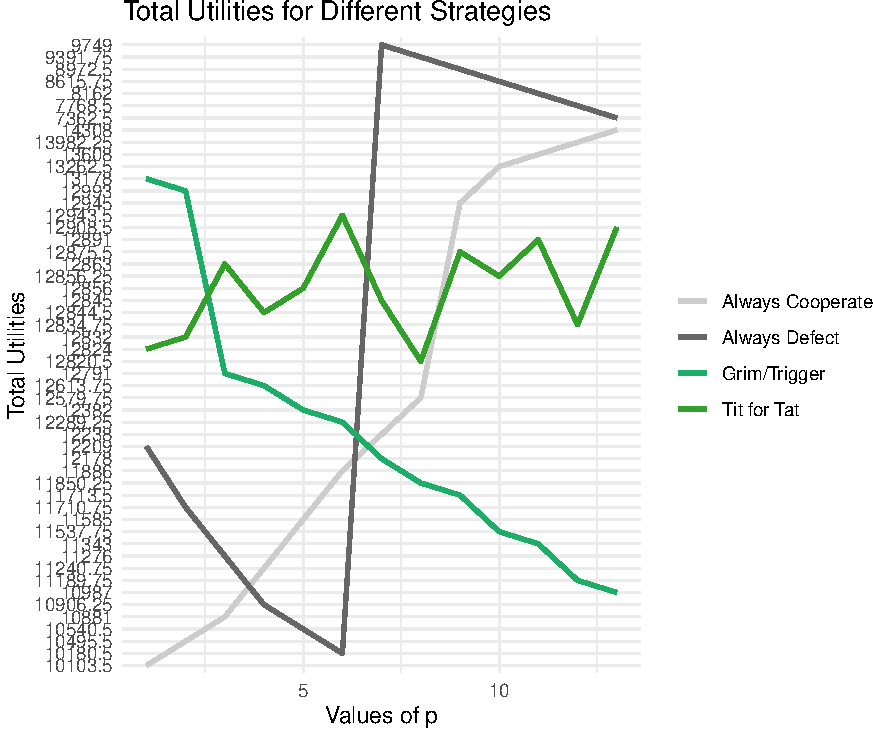
\includegraphics{Prisoners-Dilemma_files/figure-latex/unnamed-chunk-7-1} 

}

\caption{Strategy Ranks Across Different Values of p\label{pvalues}}\label{fig:unnamed-chunk-7}
\end{figure}

Defector Strategies Definition: These strategies lean towards defection
more often than cooperation. They may defect unconditionally,
strategically exploit others, or only cooperate under very specific
conditions. Defector strategies prioritize short-term gains, aiming to
maximize their own payoff without much regard for fostering mutual
cooperation.

Cooperative Strategies Definition: These strategies favour cooperation
and are designed to foster mutual cooperation over multiple rounds. They
aim to achieve better outcomes for both players through sustained
cooperation, but they often include some mechanisms for retaliation to
avoid being exploited.

Increased Temptation: c(3, 8, 0, 1) Reduced Punishment: c(3, 5, 0, 2)
Increased Reward for Cooperation: c(5, 3, 0, 1)

Increased Temptation: c(3, 8, 0, 1) This structure provides a strong
test of a strategy's ability to resist short-term gains for long-term
benefits. It is particularly useful for identifying strategies that are
susceptible to exploitation.

Reduced Punishment: c(3, 5, 0, 2) This structure will encourage more
risk-taking behavior, as the consequences of mutual defection are less
severe. It is a good way to evaluate how strategies respond to a less
punishing environment.

Increased Reward for Cooperation: c(5, 3, 0, 1) This structure will test
a strategy's ability to incentivize and maintain cooperation, even when
the temptation to defect remains. It is especially useful for
identifying strategies that are effective in promoting mutual benefit.

\section{Bump Chart}\label{bump-chart}

\newpage

\section*{References}\label{references}
\addcontentsline{toc}{section}{References}

\phantomsection\label{refs}
\begin{CSLReferences}{1}{1}
\bibitem[\citeproctext]{ref-axelrod1980effective}
Axelrod, R. 1980. Effective choice in the prisoner's dilemma. \emph{The
Journal of Conflict Resolution}. 24(1):3--25. {[}Online{]}, Available:
\url{http://www.jstor.org/stable/173932}.

\bibitem[\citeproctext]{ref-dalbo2019strategy}
Bó, P.D. \& Fréchette, G.R. 2019.
\href{https://doi.org/10.1257/aer.20181480}{Strategy choice in the
infinitely repeated prisoner's dilemma}. \emph{American Economic
Review}. 109(11):3929--3952.

\bibitem[\citeproctext]{ref-breitmoser2015cooperation}
Breitmoser, Y. 2015.
\href{https://doi.org/10.1257/aer.20130675}{Cooperation, but no
reciprocity: Individual strategies in the repeated prisoner's dilemma}.
\emph{American Economic Review}. 105(9):2882--2910.

\bibitem[\citeproctext]{ref-embrey2017cooperation}
Embrey, M., Fréchette, G.R. \& Yuksel, S. 2018.
\href{https://doi.org/10.1093/qje/qjx033}{Cooperation in the finitely
repeated prisoner's dilemma}. \emph{The Quarterly Journal of Economics}.
133(2):509--551.

\bibitem[\citeproctext]{ref-farrell1988evolutionary}
Farrell, J. \& Ware, R. 1989. Evolutionary stability in the repeated
prisoner's dilemma. \emph{Journal of Economic Theory}. 47(1):1--12.

\bibitem[\citeproctext]{ref-garcia2018no}
García, J. \& Veelen, M. van. 2018.
\href{https://doi.org/10.3389/frobt.2018.00102}{No strategy can win in
the repeated prisoner's dilemma: Linking game theory and computer
simulations}. \emph{Frontiers in Robotics and AI}. 5:102.

\bibitem[\citeproctext]{ref-gaudesi2016exploiting}
Gaudesi, M., Piccolo, E., Squillero, G. \& Tonda, A. 2016. Exploiting
evolutionary modeling to prevail in iterated prisoner's dilemma
tournaments. \emph{IEEE Transactions on Computational Intelligence and
AI in Games}. 8(3):235--247.

\bibitem[\citeproctext]{ref-kreps1982rational}
Kreps, D.M., Milgrom, P., Roberts, J. \& Wilson, R. 1982. Rational
cooperation in the finitely repeated prisoners' dilemma. \emph{Journal
of Economic Theory}. 27(2):245--252.

\bibitem[\citeproctext]{ref-lange2007teaching}
Lange, C. \& Baylor, A.L. 2007.
\href{https://doi.org/10.3200/JECE.38.4.407-418}{Teaching the repeated
prisoner's dilemma with a computerized tournament}. \emph{The Journal of
Economic Education}. 38(4):407--418.

\bibitem[\citeproctext]{ref-romero2018constructing}
Romero, J. \& Rosokha, Y. 2018.
\href{https://doi.org/10.1016/j.euroecorev.2018.02.008}{Constructing
strategies in the indefinitely repeated prisoner's dilemma game}.
\emph{European Economic Review}. 104:185--219.

\end{CSLReferences}

\bibliography{Tex/ref}





\end{document}
